\section{Results of DWBA post-form calculations}\label{sec:post}

\begin{figure}[t]
	\centering
	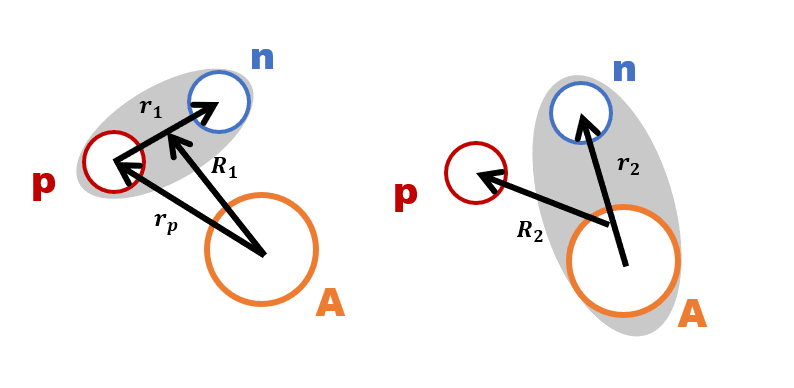
\includegraphics[width=0.80\textwidth]{transfer.png}
	\caption{Coordinates used in one neutron transfer reaction. }
	\label{fig:transfer}
\end{figure}
In a transfer reaction A(d,p)B showed in Fig. \ref{fig:transfer}, by introduction the auxiliary potential $U_f(R_2)$, the transfer T-matrix has a formula \cite{thompson2009nuclear}
\begin{equation}\label{eq:postexact}
	T_{\mathrm{post}}=\langle\phi_{nA}\chi_{pB}^{(-)}\left|V_{np}(r_1)+U_{pA}(r_p)-U_f(R_2)\right|\Psi_1^{(+)}(\vec{r}_1,\vec{R}_1)\rangle,
\end{equation}
where $\phi_{nA}$ and $\chi_{pB}$ are bound states wave-functions. 
Under first-order DWBA, it becomes
\begin{equation}\label{tpost}
	T_{\mathrm{post}}^{\mathrm{DWBA}}=\langle\phi_{nA}\chi_{pB}^{(-)}\left|V_{np}(r_1)+U_{pA}(r_p)-U_f(R_2)\right|\phi_{np}\chi_{dA}\rangle.
\end{equation}
Besides that, we still need information for the auxiliary potential $U_f(R_2)$. 
It's usually chosen as $U_{pB}(R_2)$ fitted from elastic scattering.
We name $V_{np}(r_1)$ as binding potential and the rest two remnants.

Here are three different handling methods we used in our calculations.
\begin{enumerate}
\item Zero range (ZR) approximation: Remnants are neglected; $V_{np}(r_1)$ is considered as a local interaction with strength $D_0$.
	Correspondingly, the T-matrix becomes
	\begin{equation}
		T_{\mathrm{post}}^{\mathrm{ZR-DWBA}}=D_0\langle\phi_{nA}(R_1)\chi_{pB}^{(-)}| \chi_{dA}(R_1)\rangle.
	\end{equation}
	It now relies on $R_1$ only, which simplifies calculation.
	\item First-order DWBA: finite-range interactions, without and with full complex remnant. The former abandons the remnants but the latter keeps them. The nonlocality of $V_{np}(r_1)$ is preserved in both.
\end{enumerate}

 \begin{figure}[tb]
    \begin{subfigure}{0.5\textwidth}
		\centering
		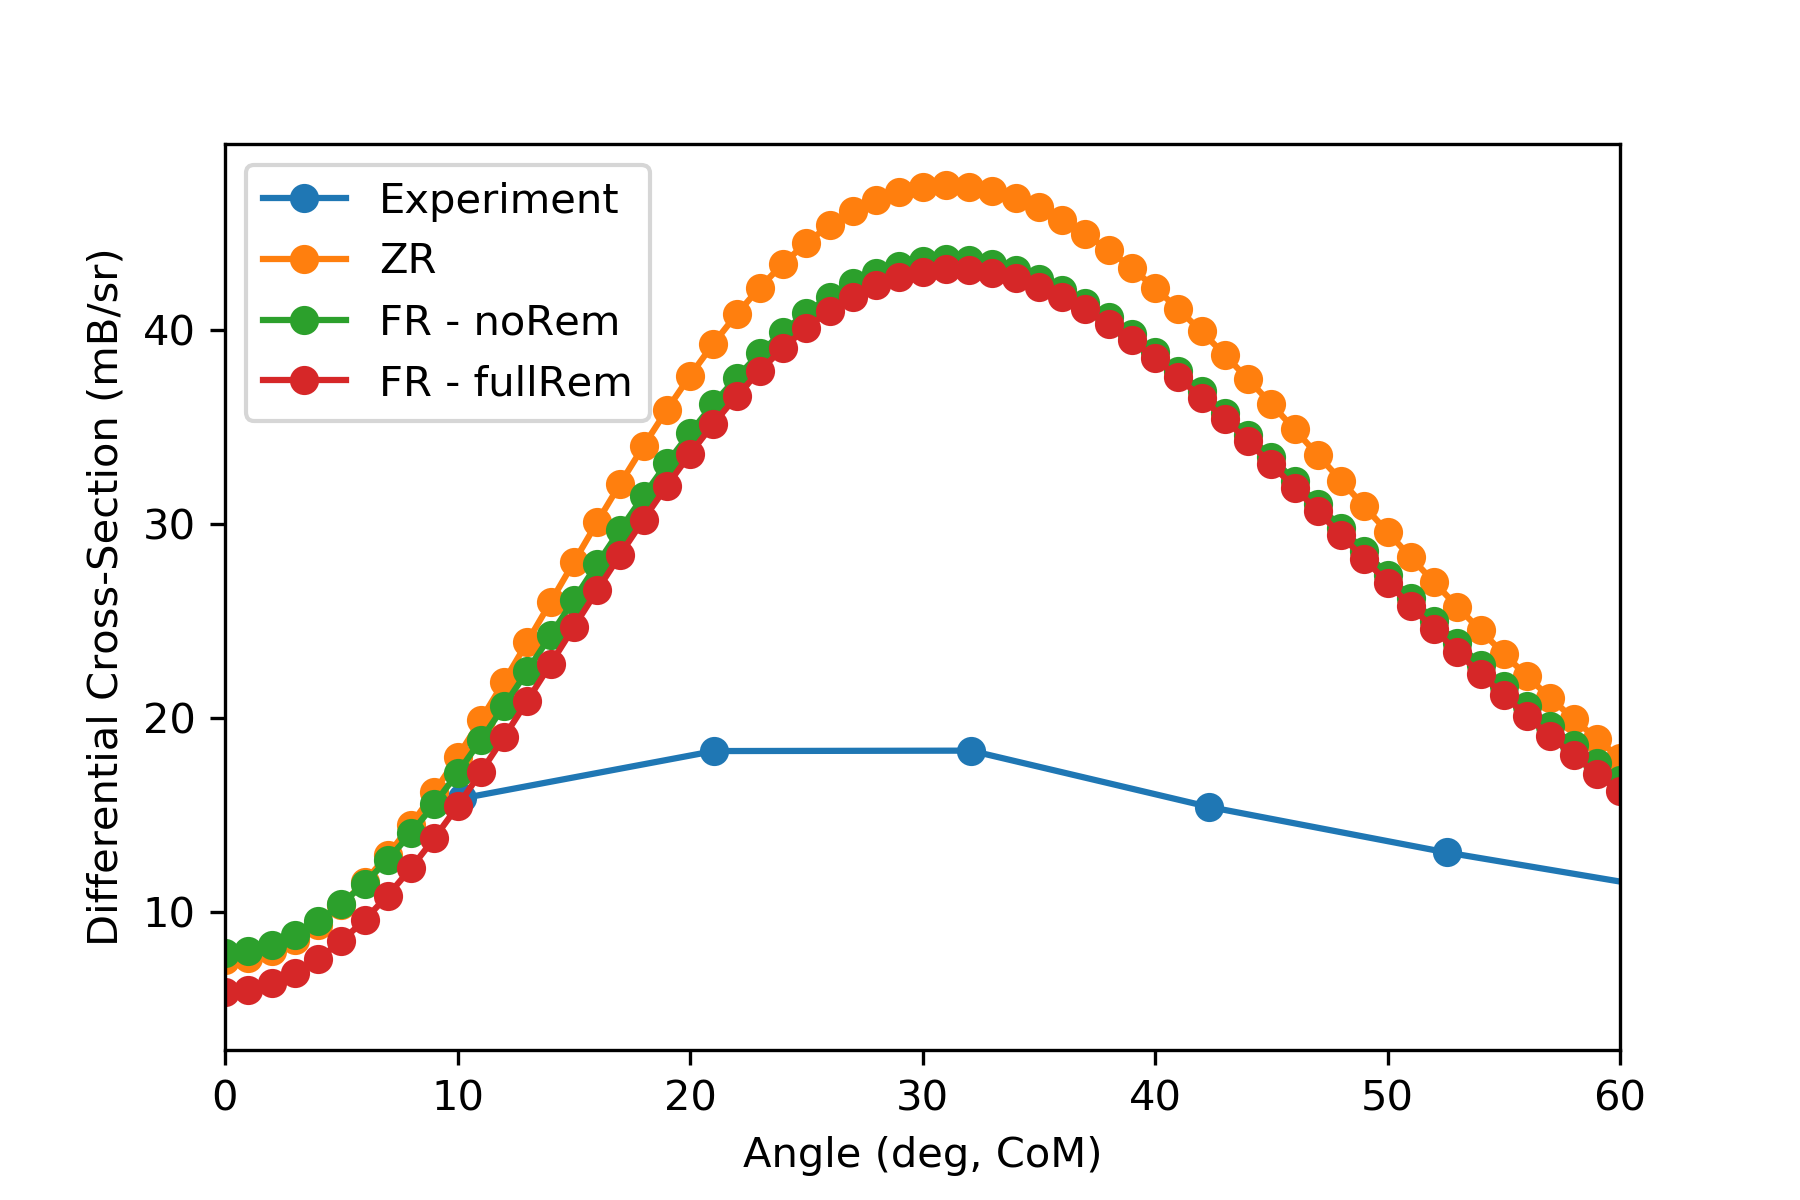
\includegraphics[width=0.98\textwidth]{3MeVReactions.png}
		\caption{Beam energy is 2.84 MeV. }
		\label{fig:3MeV}
	\end{subfigure}
        \begin{subfigure}{0.5\textwidth}
		\centering
		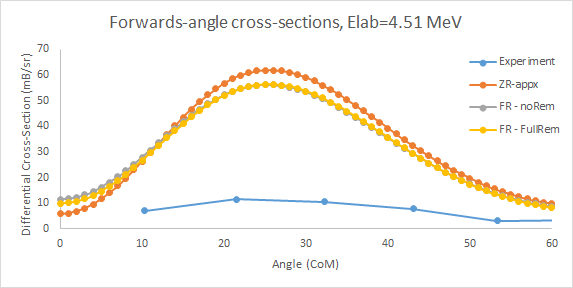
\includegraphics[width=0.98\textwidth]{5MeVReactions.png}
		\caption{Beam energy is 4.51 MeV.}
		\label{fig:5MeV}
        \end{subfigure}
       \caption{Forward-angled differential cross sections calculated under: 1) zero-range approximation (ZR); 2) first-order DWBA in post form, finite range, without remnant (FR - noRem); 3) first-order DWBA in post form, finite range, with full complex remnant (FR - fullRem), as well as experimental data. }
        	%Left and right panels are for 2.84 MeV and 4.51 MeV, repectively.}
        \label{fig:post}
  \end{figure}

Our results are generated with radius $r_{\mathrm{match}}$ = 60 fm, partial waves up to $j_{\max}$ = 55 (in units of $\hbar$) and step size $rintp$ = 0.2 fm. 
Under zero-range approximation, coefficient $D0$ is chosen to be 125.35 MeV, the same as FRESCO's recommendation. 
To test the convergence, these values are modified up to $r_{\mathrm{match}}$ = 80 and $j_{\max}$ = 70 and down to $rintp$ = 0.01 for the full complex remnant case.
 The differential cross sections deviate $<$ 2$\%$  between calculation initializations. 
 Furthermore, as long as $rintp >$ 0.05, the deviation from primary initializations is $<$ 0.5$\%$, so $< 2\%$ is a conservative limit to stability. 
 Other grid and strength parameters like non-local range $rnl$ and $centre$ are adapted from FRESCO's suggestions,
while $rnl$ is set to 0.5 fm larger than the largest $rnl$ suggestion.

The post-form results together with experimental data \cite{PhysRev.101.209} are presented in Fig. \ref{fig:post}.
In both energy scales, all three differential cross sections fit well with experiment in shape. 
Also, the agreement is better for 4.51 MeV case, as it gives more direct reactions than the 2.84 MeV case.
We can see that ZR approximation gives result deviates most from experiment because it applies the roughest approximation.
It looks DWBA with or without remnants yield very similar results.
This is anticipated because of the similarity in $U_{pA}$ and $U_{pB}$ that they almost cancel each other in Eq. \ref{tpost}.
However, DWBA with remnants is closer to experiment, which is not surprising. 